\documentclass{article}


\usepackage{arxiv}

\usepackage[utf8]{inputenc} % allow utf-8 input
\usepackage[T1]{fontenc}    % use 8-bit T1 fonts
\usepackage{hyperref}       % hyperlinks
\usepackage{url}            % simple URL typesetting
\usepackage{booktabs}       % professional-quality tables
\usepackage{amsfonts}       % blackboard math symbols
\usepackage{nicefrac}       % compact symbols for 1/2, etc.
\usepackage{microtype}      % microtypography
\usepackage{lipsum}
\usepackage{graphicx} %package to manage images
\graphicspath{ {./images/} }

\usepackage[rightcaption]{sidecap}

\usepackage{wrapfig}
\title{Algorithmic Discrimination and AI Fairness 360}


\author{
  Ashar Farooq\\
  Department of Electrical Engineering and Computer Science\\
  Massachusetts Institute of Technology\\
  Cambridge, MA 02139 \\
  \texttt{afarooq@mit.edu} \\
  %% \AND
  %% Coauthor \\
  %% Affiliation \\
  %% Address \\
  %% \texttt{email} \\
  %% \And
  %% Coauthor \\
  %% Affiliation \\
  %% Address \\
  %% \texttt{email} \\
  %% \And
  %% Coauthor \\
  %% Affiliation \\
  %% Address \\
  %% \texttt{email} \\
}

\begin{document}
\maketitle
\begin{abstract}
Algorithmic discrimination is a large issue in many domains in the modern world where computation and automation are desirable tools. With many corporations and individuals developing advanced algorithms, there is bound to be statistically significant inaccuracies if fairness is not taken into serious consideration. Specifically, machine learning algorithms that are only so much human dependent can and have created biases in algorithmic processing. To this end, IBM has developed an open source fairness toolkit entitled AI Fairness 360(AIF360). This is an important step in empowering corporations and individuals to detect bias, utilize a bias mitigation algorithm, and compare the said results to determine the effectiveness of the process. 
\end{abstract}



\section{Introduction}
There has been much research done into algorithmic discrimination, resulting in various techniques to make more equitable algorithms and subsequent predictions based on the produced models. Some of these bias mitigation techniques have been integrated into the AI Fairness 360(AIF360) toolkit as this is an open source project. AI Fairness 360(AIF360) allows anyone to utilize several bias mitigation algorithms and fairness metrics in order to analyze and mitigate biases. 
\\

This paper is organized as follows. In Section 2, I provide explanations of various terminologies specific to the context of algorithmic discrimination and AI Fairness 360(AIF360). In Section 3, I present the implications of bias in data. In Section 4, I detail the legal framework in the context of algorithmic fairness. In Section 5, I present the structure and usage of the open source state of the art AI Fairness 360(AIF360) toolkit. In Section 6, I present an example of algorithmic discrimination in the criminal justice domain and the usage of the AI Fairness 360(AIF360) toolkit in order to mitigate bias. In Section 7, I present an example of a hypothetical scenario that showcases a tradeoff between making a model accurate versus making a model legal. I also discuss potential ways of proceeding with this scenario. In Section 8, I explain the effectiveness of the toolkit. In Section 9, I present the notion of algorithmic auditing and its importance for the future. In Section 10, I note various literature on algorithmic discrimination and big data. Potential future legal considerations and concluding remarks are detailed in Sections 11 and 12, respectively. 



\section{Terminology}

In this section, I explain various terminologies associated with algorithmic discrimination and AI Fairness 360(AIF360). \textit{Bias} is defined as a fundamental error resulting in an underprivileged setting for a particular group or individual. \textit{Group fairness} is described as particular groups receiving the same standard of treatment. \textit{Individual fairness} is described as particular similar individuals receiving the same standard of treatment.  \textit{Protected attributes} are features that are prohibited categories to discriminate upon, including, but not limited to, race, gender, religion, and sexual orientation. \textit{Fairness metric} is a mathematical measurement that statistically defines bias in a model or dataset. There are approximately 70 fairness metrics utilized in AI Fairness 360(AIF360) as of the date of this written paper, including, but not limited to, Statistical Parity Difference, Mean Difference, Average Odds Difference, and Manhattan Difference. \textit{Bias mitigation algorithm} is defined to be a process that removes unwanted bias and works to better the measurement of the fairness metrics. There are approximately 10 bias mitigation algorithms utilized in AI Fairness 360(AIF360) as of the date of this written paper, including, but not limited to, Optimized Pre-processing, Prejudice Remover Algorithm, Adversarial Debiasing, and Reject Option Classification. 

\section{Data and Bias}

Much of the bias that results in algorithmic discrimination and inaccurate models is derived from misleading or inaccurate data. 

\subsection{Data}

Authentic datasets are often large and improperly formatted for AI Fairness 360(AIF360). Therefore, the dataset should be correctly integrated for use with the AI Fairness 360(AIF360) toolkit. Without such proper care, there is a statistically significant probability of added bias in the data utilized for training a model, thus leading to inaccurate predictions. I define \textit{accurate data} to be authentic data that is measured, observed, calculated, and/or derived from the real world. I define \textit{good representative data} to be not undersampled and not oversampled. This is a critical prerequisite for accurate and useful model predictions in the machine learning process. I define \textit{good data} to be both accurate data and good representative data. The lack of good data can lead to bias. 

\subsection{Bias}

One type of bias that dictates a lack of good data is \textit{sample bias}. This occurs due to accurate data and not good representative data. This can cause a fundamental error towards a particular group as this data is not a good representation of the different stakeholders and parts of the real world. With bad sampling, the machine learning algorithm will train on perhaps a particular subset of data that is not representative of the truth, which is a fundamental flaw resulting in bias. 
$\newline$

Another type of bias that dictates a lack of good data is \textit{inaccurate data bias}. In this setting, the data provided to the machine learning algorithm has been altered or is simply not accurate, thus not representing the truth. This will lead to further bias. 
$\newline$

Even with the lack of sample bias and inaccurate data bias, data can still exhibit \textit{prejudice bias}. This is the result of the history of inequity to certain groups, leading to data that is not truly representative of the potential of the stakeholders in the present day. This bias can be harder to track and can lead to implicit biases due to the representation of historical discrimination present in the data.
$\newline$

One possible bias mitigation technique for prejudice bias is augmenting the training data. In this scenario, copying the data and inverting the biases within the data can effectively eliminate the overall bias due to historical discrimination, thus the model would not make biased predictions.

\section{The Law}

The \textit{Civil Rights Act of 1964} prohibits discrimination based on certain protected attributes, including, but not limited to, race, sex, religion, age for workers over 40 years old, national origin, and pregnancy. 
$\newline$

The United States legal system distinguishes between intentional and unintentional discrimination. Disparate treatment refers to intentional discrimination based on certain protected attributes. This is in violation of civil rights legislations. Disparate impact refers to unintentional discrimination that results due to a certain unforeseen impact of a decision. This is deemed against the law unless the party can prove that such classification feature is necessary for the requirements and success of such party. The United States Supreme Court ruled in \textit{Griggs v. Duke Power Co.} that pre-employment tests needed to be justified for the success and betterment of the job placement. 
$\newline$

The Four-Fifths Rule, also known as the 80\% Rule, states the presence of an adverse impact on a particular group if the rate of selection of this particular group is less than 80\% than another group of higher rate of selection. 

\section{Overall Structure and Usage of AI Fairness 360}

AI Fairness 360(AIF360) deals with a standard machine learning process. The initial dataset after being formatted appropriately is randomly split into training data and test data. The purpose of the training data is to allow the machine learning algorithm to learn the correlations and produce a model to allow for predictions. The purpose of the test data is to compare it with the model outcomes to determine the accuracy of the model as a check. Bias can enter in three stages during the machine learning process: in the training data, in the algorithm, in the test data/predictions. If there is a biased training data as determined by a fairness metric, then a pre-processing algorithm, such as Optimized Pre-processing, can be utilized. If the machine learning process of classification is biased, then an In-processing algorithm, such as Adversarial Debiasing, can be utilized. If there is bias in the predicted values and test data, then a Post-processing algorithm, such as the Equalized Odds Post-processing algorithm, can be utilized. 
$\newline$

Using AI Fairness 360(AIF360) can require simply 5 steps. The first step in utilizing the AI Fairness 360(AIF360) toolkit is to import the necessary packages and dataset. The next step is to split the loaded dataset into training data and testing data. The 3rd step is to determine the measurement of a fairness metric on the original training data. The next step after consists of utilizing a bias mitigation algorithm. The final step is to compute the said fairness metric on the dataset and analyze the changes. 

\section{COMPAS Example}

COMPAS, which stands for Correctional Offender Management Profiling for Alternative Sanctions, is an algorithmic tool utilized in the criminal justice system in order to evaluate a defendant’s likelihood of reoffending. This tool has been criticized heavily for determining a higher recidivism score for African American defendants twice as likely as compared to other defendants. Fairness metrics utilized in the AI Fairness 360(AIF360) toolkit shows statistically significant bias against African American defendants in many instances. 
$\newline$

The AI Fairness 360(AIF360) toolkit can be utilized here to mitigate bias. It is important to note that making model predictions based on the protected attribute of race is against the law. Due to the trade secret of the COMPAS algorithm, there is much uncertainty regarding the workings of the algorithm. 
$\newline$

One specific way that the AI Fairness 360(AIF360) toolkit can mitigate the bias against African American defendants is through the Adversarial Debiasing algorithm. This bias mitigation technique analyzes and iterates over the training data in order to potentially predict a protected attribute, such as race in the case of the COMPAS example. If this algorithm can indeed predict the attribute, then this suggests that the model will take race into account, which has negative implications for the African American defendants, perhaps due to the historical systemic racism and police brutality against African Americans. Adversarial Debiasing will remove the biased correlation from the dataset, thus the machine learning process will be equitable. This will lead to accurate predictions that do not penalize African American defendants due to the color of their skin. 

\begin{center}
  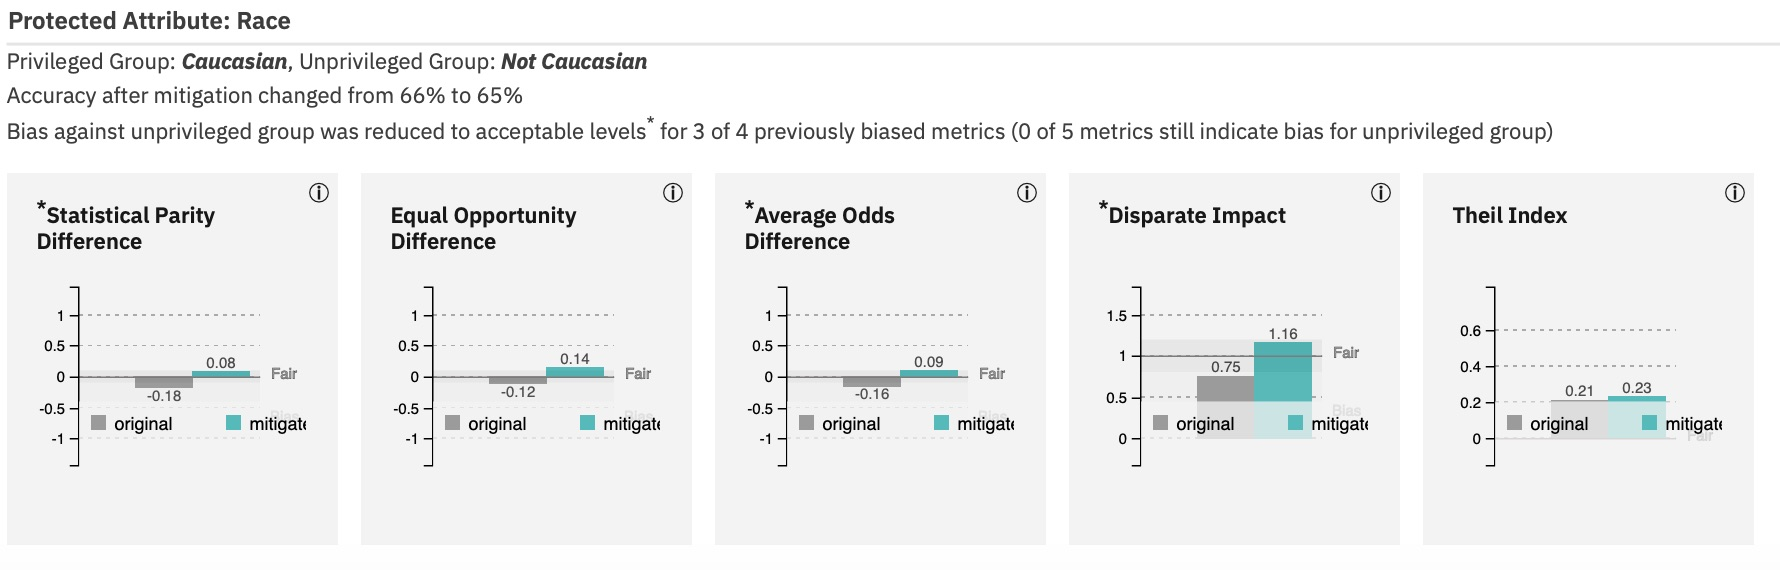
\includegraphics[width=1.0\textwidth]{COMPAS.jpg}
  \caption{This is a web demonstration of the effects of the AI Fairness 360(AIF360) toolkit. Using a sample COMPAS dataset and the protected attribute of race, the bias against African American defendants has been heavily reduced after the adversarial debiasing bias mitigation algorithm is utilized. }
\end{center}

\section{Tradeoff Between Legality and Accuracy}

There are certain examples where making the machine learning model accurate will make the predictions illegal and vice versa. This challenge between machine learning and the legal system is exhibited in the following hypothetical example:
$\newline$

Assume the following:

\begin{itemize}
\item It is illegal to discriminate against workers over 40 under the \textit{Age Discrimination in Employment Act}, and that discrimination can take the form of disparate impact.
\item A job requires lifting 75 pounds.
\item Applicants are being screened by an artificial intelligence algorithm.
\item The training data accurately shows a strong correlation between age and an inability to lift 75 pounds.
\end{itemize}
$\newline$
The challenge presented by this example is the need to not utilize a protected attribute or a proxy of a protected attribute for this would be against the law while also making the model accurate as this protected attribute is a decent predictor of successful candidates. There are many possible scenarios to proceed with this example. Sections 7.1 through Sections 7.6 detail primarily technological scenarios to this challenge while Sections 7.7 and 7.8 detail primarily societal scenarios. 

\subsection{Changing Weighted Parameters}

In order to not utilize a protected attribute heavily, one scenario for this problem is to change the weighted parameters of the correlations within the training data in order to minimize the controversial correlation of a protected attribute with the outcome while keeping the other correlations with non-protected attributes as is or higher, depending on a legally optimal level. The other features used besides the protected attribute can be added to the original dataset if and when appropriate via collecting more data. 

\subsection{Unsupervised Machine Learning}

Unsupervised machine learning is the algorithm determining different relationships without the supervision of pre-classified features. The use of this method without protected attributes in the training data can help a party determine the other non-protected attributes that are also critical to getting the best candidates from a large group. After the unsupervised machine learning presents many different correlations and insights, the party can determine the useful attributes to use in the consideration of employees while not utilizing any protected attribute. This would be a legal scenario and can provide further correlations in order for the party to perform a holistic review of an applicant since the party should not decide job placement only based on the correlation between age and an inability to lift 75 pounds. 

\subsection{Reinforcement Machine Learning}

Reinforcement machine learning trains a model on the basis of positive reward for making the correct predictions and negative reward for making inaccurate predictions, eventually leading to the model that the party desires. This method can be utilized in this example by giving a reward for correctly identifying a good candidate(as measured by someone actually being able to lift 75 pounds) and negative reward for not identifying a good candidate(as measured by someone not being able to lift 75 pounds). In this machine learning process, there are no protected attributes if desired or lightly weighted protected attributes if desired. Over time, the machine learning model will determine various correlations between certain non-protected attributes, thus utilizing them in the machine learning model to screen candidates in a legal procedure. 

\subsection{Minimizing Loss Function}

Loss function can be described as numerical error that can be measured by the number of incorrect model predictions. In this example, the loss function is a quantitative representation of the correlation between the model predictions to the protected attribute age. Minimizing the loss function would cause the machine learning model to learn the lack of importance of age in this model, thus not utilizing the protected attribute age as much. The model would stop or strongly decrease the correlation between age and an inability to lift 75 pounds. Instead, the model would depend more on other non-protected attributes to make predictions. The tradeoff in this scenario is that the decrease in this correlation renders the model more inaccurate, thus an optimal legal and computationally reasonable solution is desired. 

\subsection{Minimizing Biased Subspace}

This example can be represented as a mathematical n-dimensional vector space of various correlations that the algorithm utilizes to make model predictions. Through an iterative procedure, the discriminatory component of the entire region of space can be determined as this subspace represents the biased correlation between age and an inability to lift 75 pounds. Minimizing the component that encodes this subspace can reduce the correlation between age and an inability to lift 75 pounds, effectively making the machine learning process more equitable. 

\subsection{Utilizing a Second Model}

A second model can check where in the original machine learning process bias was introduced. Through bias mitigation algorithms, the original machine learning process can be debiased, leading to more equitable predictions. 


\subsection{Holistic Review}

In this societal scenario, the use of a protected attribute, such as age, as only one factor from among many other non-protected factors can be a socially optimal solution. These other factors can also be more heavily weighted within an optimal legal threshold. In this approach, the model will produce more equitable outcomes, which can inform the party of a single factor that can be used to make decisions within a holistic review of a candidate.

\subsection{Collecting More Data}

If appropriate, collecting further data that includes more non-protected attributes can help improve the accuracy of the machine learning model while also providing a legal approach to making decisions. 

\section{Effectiveness of AI Fairness 360}

The AI Fairness 360(AIF360) toolkit is overall fairly effective in various domains. It is user-friendly, simple, and widely accessible. However, it is limiting in its scope to risk assessment or allocation settings. In addition, the open source toolkit also has a prerequisite of having appropriate protected attributes and a numeral definition of fairness. 

\section{Algorithmic Auditing}

With the rapid development of complicated algorithms whose implementation details are a black box due to trade secret regulations, the need for algorithmic auditing is expected to increase. Algorithmic auditing revolves around feeding an algorithm various specific inputs and analyzing the outputs. The auditing process also notes various aspects of the algorithm, including accuracy, transparency, fairness, legal conformity, and evidence of bias. Algorithmic auditing by an independent organization can lead to better trust between consumers and algorithmic powerhouses. 

\section{Literature on Algorithmic and Big Data Discrimination}

Various literature on the topics of algorithmic discrimination and big data is present. Prominent pieces include, but are not limited to, Cathy O’Neil’s \textit{Weapons of Math Destruction: How Big Data Increases Inequality and Threatens Democracy}, Safiya Noble’s \textit{Algorithms of Oppression: How Search Engines Reinforce Racism}, Meredith Broussard’s \textit{Artificial Unintelligence: How Computers Misunderstand the World}, Andrew G. Ferguson’s \textit{The Rise of Big Data Policing: Surveillance, Race, and the Future of Law Enforcement}, and Virginia Eubanks’s \textit{Automating Inequality: How High-Tech Tools Profile, Police, and Punish the Poor}.

\section{Future Legal Scenarios To Consider}

The intersection of the law and artificial intelligence is expected to generate many challenges. Two hypothetical examples are presented for future considerations. 
$\newline$

Suppose younger people(less than 40 years old) are more correlated with better academic success than older people(over 40 years old) and that equal number of people apply for college admissions. Can people or artificial intelligence use age to select more qualified candidates even if using the protected attribute age is illegal? What would they do?
$\newline$

Suppose there are many qualified people living in Washington D.C for a political job(strong correlation). Can people or artificial intelligence use zip code location(a proxy for protected attribute race) to select more qualified candidates if using a proxy for race is illegal? What would they do?

\section{Conclusion}

Algorithmic discrimination is a challening and complicated problem to alleviate. Bias can be introduced in the machine learning process by an improper method of collecting data, leading to an ill-representative data or inaccurate data. Data can also contain prejudice bias as a result of historical discrimination. The machine learning algorithm can also be biased as can the testing data. 
$\newline$

The AI Fairness 360(AIF360) toolkit is a simple tool for determining, analyzing, and removing unwanted bias. The measure of the bias via many fairness metrics can illustrate the effectiveness of the many bias mitigation algorithms utilized on the toolkit. 
$\newline$

In many instances, there are legal implications that make it more challenging to have an accurate model that also complies with legal requirements. There are various technological and societal methods of proceeding with these challenges. In the future, more research into algorithmic discrimination, big data, fairness, and other bias mitigation toolkits are necessary for the more challenges on the horizon. 


\bibliographystyle{unsrt}  
%\bibliography{references}  %%% Remove comment to use the external .bib file (using bibtex).
%%% and comment out the ``thebibliography'' section.


%%% Comment out this section when you \bibliography{references} is enabled.
\begin{thebibliography}{1}

\bibitem{bellamy2018ai}
Brian Hu Zhang, Blake Lemoine, and Margaret Mitchell
\newblock Mitigating Unwanted Biases with Adversarial Learning.
\newblock {\em  AAAI/ACM Conference on Artificial Intelligence, Ethics, and Society}, 2018.

 \bibitem{bellamy2018ai}
 Faisal Kamiran, Asim Karim, and Xiangliang Zhang.
\newblock Decision Theory for Discrimination-Aware Classification.
\newblock {\em  IEEE International Conference on Data Mining}, 2012.

\bibitem{bellamy2018ai}
IBM.
\newblock AI Fairness 360 Open Source Toolkit.
\newblock {\em  aif360.mybluemix.net/.}

\bibitem{bellamy2018ai}
Michael Feldman, Sorelle A. Friedler, John Moeller, Carlos Scheidegger, and Suresh Venkatasubramanian.
\newblock Certifying and Removing Disparate Impact.
\newblock {\em  ACM SIGKDD International Conference on Knowledge Discovery and Data Mining}, 2015.

\bibitem{bellamy2018ai}
Rachel K. E. Bellamy and Kuntal Dey and Michael Hind and Samuel C. Hoffman and Stephanie Houde and Kalapriya Kannan and Pranay Lohia and Jacquelyn Martino and Sameep Mehta and Aleksandra Mojsilovic and Seema Nagar and Karthikeyan Natesan Ramamurthy and John Richards and Diptikalyan Saha and Prasanna Sattigeri and Moninder Singh and Kush R. Varshney and Yunfeng Zhang.
\newblock AI Fairness 360: An Extensible Toolkit for Detecting, Understanding, and Mitigating Unwanted Algorithmic Bias.
\newblock {\em arXiv eprint arXiv:1810.01943}, 2018.

\end{thebibliography}


\end{document}



\begin{center}
  \url{https://www.ctan.org/pkg/booktabs}
\end{center}
See Figure \ref{fig:fig1}. Here is how you add footnotes. \footnote{Sample of the first footnote.}

